\begin{enumerate}[label=\thesubsection.\arabic*, ref=\thesubsection.\theenumi]


    \item The value(s) of k for which the quadratic equation $2x^2 + kx + 2 = 0$ has equal roots, is
\begin{enumerate}
	\begin{multicols}{4}
\item  4

\item $\pm 4$

\item  -4

\item  0 
\end{multicols}
\end{enumerate}

\solution 

For a quadratic equation $ ax^2+bx+c=0$,condition to have equal roots 

from \eqref{eq:EE26BTECH11222-prob 1}
\begin{align}
b^2-4ac=0    
\end{align}

$k^2-16=0 \implies k=\pm 4$

\begin{align}
	\textbf{codes/10/q1.py}
\end{align}
   \item which of the following is not an A.P?
   \begin{enumerate}
   	

\item -1.2,0.8,2.8 ...

\item$3,3+\sqrt{2},3+2\sqrt{2},....$

\item$\frac{4}{3},\frac{7}{3},\frac{9}{3},\frac{12}{3}...$

\item$\frac{-1}{5},\frac{-2}{5},\frac{-3}{5}....$


\end{enumerate}
\solution 

a.$a_2-a_1= 2,a_3-a_2=2 $, so,they form an A.P with common difference 2

b.$a_2-a_1=\sqrt{2}, a_3-a_2=\sqrt{2}$ , they form an A.P with common difference $\sqrt{2}$

c.$a_3-a_2=\frac{2}{3},a_4-a_3=1$, no common difference ,so they doesn't form an A.P

\item The radius of a sphere (in cm) whose volume is $12\pi\text{ cm}^{3}$ is
  \begin{enumerate}
			\begin{multicols}{4}
				\item 3

\item$3\sqrt{3}$

\item $3^{2/3}$

\item $3^{1/3}$
\end{multicols}
\end{enumerate}
\solution 

from \eqref{eq:EE26BTECH11222-prob 3}

volume of the sphere

\begin{align}
    V=\frac{4}{3}\pi r^3 cm^3 
\end{align}
$\frac{4}{3}\pi r^3 = 12 \pi cm^3 \implies r= 3^{\frac{2}{3}} cm $

\item The distance between the points $(m, -n)$ and $(-m, n)$ is
\begin{enumerate}
	\begin{multicols}{4}
\item $\sqrt{m^{2}+n^{2}}$ 

\item $m+n$ 

\item $2\sqrt{m^{2}+n^{2}}$  

\item $\sqrt{2m^{2}+2n^{2}}$

\end{multicols}
\end{enumerate}
\solution 

from \eqref{eq:EE26BTECH11222-prob 4}

distance between two points $(x_1,y_1); (x_2,y_2)$ is 
\begin{align}
\sqrt{(x_2-x_1)^2 +(y_2-y_1)^2}    
\end{align}


distance $\sqrt{4m^2+4n^2}\implies 2\sqrt{m^2+n^2}$


\item In Figure-1, from an external point P, two tangents PQ and PR are drawn to a circle of radius 4 cm with centre O. If $\angle QPR = 90^{\circ}$, then length of PQ is 
\begin{enumerate}
	\begin{multicols}{4}

\item 3 cm

\item 4 cm

\item 2 cm

\item $2\sqrt{2}\text{cm}$
\end{multicols}
\end{enumerate}



\begin{center}
	
	\begin{tikzpicture}[scale=0.5, transform shape, thick]
		% Define coordinates
		\coordinate (O) at (0,0);
		\coordinate (Q) at (0,4);
		\coordinate (R) at (4,0);
		\coordinate (P) at (4,4);
		
		% Draw the circle
		\draw (O) circle (4cm);
		
		% Draw radius OQ with label
		\draw (O) -- (Q) node[midway, left] {$4\text{ cm}$};
		
		% Draw dashed line from O to P
		\draw[dashed] (O) -- (P);
		
		% Draw tangent lines meeting at P with arrows pointing outward
		\draw[->] (P) -- (-3,4);
		\draw[->] (P) -- (4,-3);
		
		% Right angle symbol at P
		\draw (3.7,4) -- (3.7,3.7) -- (4,3.7);
		
		\pic [draw, "$45^\circ$", angle radius=10mm, angle eccentricity=1.4] {angle = Q--P--O};
		% Draw points
		\fill (O) circle (2.5pt);
		\fill (Q) circle (2.5pt);
		\fill (R) circle (2.5pt);
		\fill (P) circle (2.5pt);
		
		% Node labels
		\node[below left] at (O) {$O$};
		\node[above right] at (Q) {$Q$};
		\node[right] at (R) {$R$};
		\node[above right] at (P) {$P$};
		
	\end{tikzpicture}
\end{center}


\solution 
The line joining the centre to the point of intersection bisects the angle between the tangents.



so $\angle {OPQ} = \frac{\pi}{4}$ $tan(\frac{\pi}{4})= \frac{OP}{PQ}$



$PQ= OP \implies PQ = 4cm$

\item On dividing a polynomial $p(x)$ by $x^{2}-4$, quotient and remainder are found to be $x$ and 3 respectively. The polynomial $p(x)$ is   
\begin{enumerate}
	\begin{multicols}{4}
		\item $3x^{2}+x-12$
		\item  $x^{3}-4x+3$ 
		\item $x^{2}+3x-4$ 
 		\item$x^{3}-4x-3$
	\end{multicols}
\end{enumerate}	
\solution 
from \eqref{eq:ee26btech11222-prob 6}

\begin{align}
	P(x)= Q(x)Y(x) +R(x) 
\end{align}

$P(x), Y(x)=x^2-4,Q(x)=x,R(x)=3$

$P(x)= x^3-4x + 3$


\item In Figure-2, $DE \parallel BC$. If $\frac{AD}{DB} = \frac{3}{2}$ and $AE = 2\cdot7\text{ cm}$, then EC is equal to
\begin{enumerate}
	\begin{multicols}{4}
\item $2\cdot0\text{ cm}$   

\item  $1\cdot8\text{ cm}$

\item  $4\cdot0\text{ cm}$

\item  $2\cdot7\text{ cm}$

	\end{multicols}
\end{enumerate}	

\begin{center}
	
		\begin{tikzpicture}[scale=0.6, transform shape, thick]
			% Define coordinates for triangle ABC and parallel line segment DE
			\coordinate (A) at (2.5, 4);
			\coordinate (B) at (0, 0);
			\coordinate (C) at (7, 0);
			
			\coordinate (D) at (1, 1.6);
			\coordinate (E) at (5.2, 1.6);
			
			% Draw the main triangle ABC
			\draw (A) -- (B) -- (C) -- cycle;
			
			% Draw the parallel line segment DE
			\draw (D) -- (E);
			
			% Node labels for vertices and points
			\node[above] at (A) {$A$};
			\node[below left] at (B) {$B$};
			\node[below right] at (C) {$C$};
			\node[left] at (D) {$D$};
			\node[right] at (E) {$E$};
			
			% Label for segment AE
			\node[above right] at ($(A)!0.5!(E)$) {$2.7\text{ cm}$};
			
		\end{tikzpicture}
	
\end{center}
\solution

Basic Proportionality theorem : If a line is drawn parallel to one side of a triangle to intersect the other two sides in distinct points, then it divides those two sides in the same ratio.

form \eqref{eq:ee26btech11222-prob_10 7}

According to the theorem , $\frac{AD}{DB}=\frac{AE}{EC}$

$\frac{2}{3}= \frac{EC}{AE} \implies EC= 1.8cm $

\item The point on the x-axis which is equidistant from $(-4, 0)$ and $(10, 0)$ is

\begin{enumerate}
	\begin{multicols}{4}
\item $(7, 0)$

\item  $(5, 0)$ 

\item  $(0, 0)$ 

\item  $(3, 0)$
	\end{multicols}
\end{enumerate}	
\solution

let ,the point be P(x,0), Q(10,0),R(-4,0) . Distance between $\vert{}PQ\vert = \vert{}PR\vert{}$ 

$\vert{}x-10\vert{} = \vert{}x+4\vert{} \implies x=3$

\item 

The centre of a circle whose end points of a diameter are $(-6, 3)$ and $(6, 4)$ is   
\begin{enumerate}
	\begin{multicols}{4}
\item $(8, -1)$   

\item  $(4, 7)$ 

\item  $\left(0, \frac{7}{2}\right)$

\item  $\left(4, \frac{7}{2}\right)$
\end{multicols}
\end{enumerate}	
\solution


centre $\implies $midpoint of end points of diameter  

centre $O(x,y)= (\frac{x_1+x_2}{2},\frac{y_1+y_2}{2}) \implies O(x,y)= (0,\frac{7}{2})$

\item 
The pair of linear equations $\frac{3x}{2} + \frac{5y}{3} = 7$ and $9x + 10y = 14$ is   
\begin{enumerate}
	
\item consistent

\item inconsistent   

\item  consistent with one solution 

\item  consistent with many solutions

\end{enumerate}	
\solution


$9x+10y= 42 $ and $9x+10y=14$, they are parallel lines , so lines are inconsistent 

\begin{align}
	\textbf{codes/10/q9.py}
\end{align}
\item In Figure-3, PQ is tangent to the circle with centre at O, at the point B. If $\angle AOB = 100^{\circ}$, then $\angle ABP$ is equal to   
\begin{enumerate}
	\begin{multicols}{4}
		\item  $50^{\circ}$ 

\item  $40^{\circ}$

\item  $60^{\circ}$   

\item $80^{\circ}$
\end{multicols}
\end{enumerate}	

\begin{center}
 
	\begin{tikzpicture}[scale=0.6, thick]
		% Define coordinates and radius
		\coordinate (O) at (0,0);
		\def\r{3} % radius of the circle
		
		% Points on the circle (angle AOB = 100°)
		\coordinate (B) at (-75:\r);
		\coordinate (A) at (185:\r);
		
		% Draw the circle
		\draw (O) circle (\r cm);
		
		% Draw triangle OAB
		\draw (O) -- (A) -- (B) -- cycle;
		
		% Tangent line at B (perpendicular to radius OB at -75°, line angle is 15° / 195°)
		\coordinate (P) at ($(B) + (195:2.5)$);
		\coordinate (Q) at ($(B) + (15:3.5)$);
		\draw[<->] (P) -- (Q);
		
		% Tick marks on the tangent line near P and Q
		\draw ($(P)+(105:0.12)$) -- ($(P)+(-75:0.12)$);
		\draw ($(Q)+(105:0.12)$) -- ($(Q)+(-75:0.12)$);
		
		% Draw angle 100° at O
		\pic [draw, "$100^\circ$", angle radius=5mm, angle eccentricity=1.4] {angle = A--O--B};
		
		% Fill points
		\fill (O) circle (1.5pt);
		\fill (A) circle (1.5pt);
		\fill (B) circle (1.5pt);
		
		% Node labels
		\node[above right] at (O) {$O$};
		\node[left] at (A) {$A$};
		\node[below right] at (B) {$B$};
		\node[below] at (P) {$P$};
		\node[below] at (Q) {$Q$};
		
	\end{tikzpicture}

\end{center}
\solution

$\angle {OAB}=\angle{OBA} = 40^{\circ}$ 

$\angle {OBP}= 90^{\circ} \implies \angle{ABP}= 50^{\circ}$    

\item Simplest form of $\frac{1+\tan^{2}A}{1+\cot^{2}A}$ is 

\solution

$$\frac{1 + \frac{sin^2A}{cos^2A}}{1+ \frac{cos^2A}{sin^2A}} \implies \frac{sin^2A}{cos^2A} $$

$$= tan^2A$$

\item If the probability of an event E happening is $0\cdot023$, then $P(\overline{E}) =$

\textbf{solution :}

$$P(E) + P(\overline{E})= 1$$

$$P(\overline{E})= 1-P(E) \implies P(\overline{E})= 0.977$$

\item A cone and a cylinder have the same radii but the height of the cone is 3 times that of the cylinder. Find the ratio of their volumes.

\solution

let $V_1$ and $V_2$ be the volumes of cone and cylinder 

$r_1=r_2;h_1=3h_2 $ $$ V_1=\frac{1}{3}\pi r_1^2h_1 $$
$$V_2= \pi r_2^2h_2 \implies \frac{V_1}{V_2} = \frac{h_1}{3h_2} = 1$$
$$ \frac{V_1}{V_2}=1$$

\item In Figure-4, a quadrilateral ABCD is drawn to circumscribe a circle. Prove that $AB + CD = BC + AD$

\begin{center}
	
	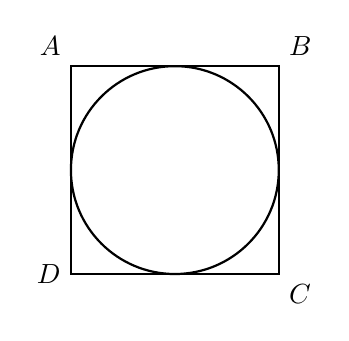
\begin{tikzpicture}[scale=0.6, thick]
		% Define the radius of the circle
		\def\r{2.2}
		
		% Draw the circle
		\draw (0,0) circle (\r cm);
		
		% Define vertices of the square circumscribing the circle
		\coordinate (A) at (-\r, \r);
		\coordinate (B) at (\r, \r);
		\coordinate (C) at (\r, -\r);
		\coordinate (D) at (-\r, -\r);
		
		% Draw the square
		\draw (A) -- (B) -- (C) -- (D) -- cycle;
		
		% Node labels for the vertices
		\node[above left] at (A) {$A$};
		\node[above right] at (B) {$B$};
		\node[below right] at (C) {$C$};
		\node[left] at (D) {$D$};
		
	\end{tikzpicture}

\end{center}
\solution

let the point of intersections of quadrilateral and circle be P,Q,R,S

side AB at P, side BC at Q, side CD at R, side AD at S

$\overline{AP}= \overline{AS} $ 

$ \overline{BP}=\overline{BQ} $,

$\overline{CQ}=\overline{CR}, $

$\overline{DR}=\overline{DS}$

$AP + PB=AB ; BQ+QC=BC ; CR+RD=CD ;DS+AS=AD$

$$AB+CD=AP+PB+CR+RD$$
$$AD+BC= AS+BQ+CQ+DS \implies AP+ PB+CR+RD$$

$$AB+CD=AD+BC$$

Hence proved .

\item 
Find the sum :
(-5)+(-8)+(-11)+ \dots +(-230)

\solution 
Find the sum of the series:
\[
(-5) + (-8) + (-11) + \dots + (-230)
\]

%\subsection*{Step 1: Identify the components of the A.P.}

 First term ($a$) = $-5$
 
 Common difference ($d$) = $(-8) - (-5) = -3$

 Last term ($l$ or $a_n$) = $-230$


%\subsection*{Step 2: Find the number of terms ($n$)}
Using the formula for the $n$-th term of an A.P., $a_n = a + (n - 1)d$:
\begin{align*}
	-230 &= -5 + (n - 1)(-3) \\
	-230 + 5 &= -3(n - 1) \\
	-225 &= -3(n - 1) \\
	n - 1 &= \frac{-225}{-3} \\
	n - 1 &= 75 \\
	n &= 76
\end{align*}

%\subsection*{Step 3: Calculate the sum of the series ($S_n$)}
Using the formula for the sum of an A.P., $S_n = \frac{n}{2}(a + l)$:
\begin{align*}
	S_{76} &= \frac{76}{2} \left[(-5) + (-230)\right] \\
	S_{76} &= 38 \times (-235) \\
	S_{76} &= -8930
\end{align*}

The sum of the given A.P. series is \mathbf{-8930}.

\item 
In Figure-5, find the perimeter of $\Delta ABC$ if AP = 12 cm

\begin{center}
	

	\begin{tikzpicture}[scale=0.6, thick]
		% Radius of the circle
		\def\r{2}
		
		% Points of tangency on the circle
		\coordinate (P) at (150:\r);
		\coordinate (Q) at (30:\r);
		\coordinate (D) at (90:\r);
		
		% Apex A at the top
		\coordinate (A) at (0, 4.8);
		
		% Draw the circle
		\draw (0,0) circle (\r cm);
		
		% Draw the main lines from A passing through P and Q extending downwards
		\coordinate (Pext) at ($(A)!1.7!(P)$);
		\coordinate (Qext) at ($(A)!1.7!(Q)$);
		\draw (A) -- (Pext);
		\draw (A) -- (Qext);
		
		% Draw the tangent line segment BC at the top of the circle passing through D
		\coordinate (B) at (-1.33, \r);
		\coordinate (C) at (1.35, \r);
		\draw (B) -- (C);
		
		% Node labels
		\node[above] at (A) {$A$};
		\node[above left] at (B) {$B$};
		\node[above right] at (C) {$C$};
		\node[above] at (D) {$D$};
		\node[left] at (P) {$P$};
		\node[right] at (Q) {$Q$};
		
	\end{tikzpicture}
\end{center}

\solution

let $BP =BD=CD=CQ= x cm $ $AP =AQ = 12cm $

$ AB = AC =12-x cm $

perimeter of $\triangle ABC = 2x+ 12-x +12-x  $

perimeter = 24cm

\item 

Find the mode of the following distribution :

\begin{tabular}{c|c|c|c|c|c|c}

\hline
marks & 0-10 & 10-20 & 20-30 & 30-40 & 40-50 & 50-60 \\ 
\hline 

number of students & 4 & 6&7&12&5 &6\\ \hline  


\end{tabular}

\solution

modal class : 30-40 

l=30 

modal frequency $(f_1)$: 12

$f_0 = 7$

$f_2= 5$

class size $h$= 10

mode = $l+ \left(\frac{f_1-f_0}{2f_1-f_0-f_2}\right)h \implies mode = 30 +\frac{25}{6}$

mode = 34.166

\item In Figure-7, if $PQ \parallel BC$ and $PR \parallel CD$, prove that $\frac{QB}{AQ} = \frac{DR}{AR}$
\begin{center}
	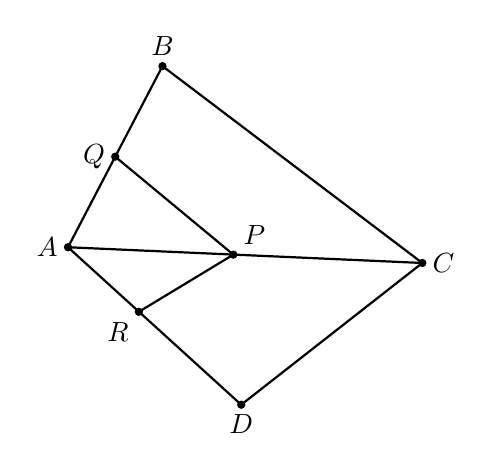
\begin{tikzpicture}[scale=1, thick]
		% Define coordinates for the vertices of quadrilateral ABCD and interior point P
		\coordinate (A) at (1, 2.5);
		\coordinate (B) at (2.2, 4.8);
		\coordinate (C) at (5.5, 2.3);
		\coordinate (D) at (3.2, 0.5);
		\coordinate (P) at (3.1, 2.406);
		
		% Define points Q on AB and R on AD (perpendicular drops from P)
		\coordinate (Q) at (1.6, 3.65);
		\coordinate (R) at (1.9, 1.68);
		
		% Draw quadrilateral ABCD
		\draw (A) -- (B) -- (C) -- (D) -- cycle;
		
		% Draw lines from interior point P to vertices and sides
		\draw (A) -- (C);
	%	\draw (P) -- (A);
	%	\draw (P) -- (B);
	%	\draw (P) -- (C);
	%	\draw (P) -- (D);
		\draw (P) -- (Q);
		\draw (P) -- (R);
		
		% Fill points
		\fill (A) circle (1.5pt);
		\fill (B) circle (1.5pt);
		\fill (C) circle (1.5pt);
		\fill (D) circle (1.5pt);
		\fill (P) circle (1.5pt);
		\fill (Q) circle (1.5pt);
		\fill (R) circle (1.5pt);
		
		% Node labels
		\node[left] at (A) {$A$};
		\node[above] at (B) {$B$};
		\node[right] at (C) {$C$};
		\node[below] at (D) {$D$};
		\node[above right] at (P) {$P$};
		\node[left] at (Q) {$Q$};
		\node[below left] at (R) {$R$};
		
	\end{tikzpicture}
\end{center}

\textbf{solution :}

For the $\triangle AQP and \triangle ABC$, given $QP ||BC$, by Thale's theorem  $\frac{AQ}{QB}=\frac{AP}{PC}$

for the $\triangle ACD and \triangle APR$, given $RP || CD$ , by Thale's theorem $ \frac{AR}{RD}=\frac{AP}{PC}$

$$\frac{AQ}{QB}=\frac{AR}{RD}$$

\item Prove that: $(\sin^{4}\theta - \cos^{4}\theta + 1)cosec^{2}\theta = 2$

\textbf{solution :}

$$((sin^2\theta -cos^2\theta)(cos^2\theta +sin^2\theta)+1)cosec^2\theta $$ $$ (1-cos(2\theta))cosec^2\theta \implies 2sin^2\theta cosec^2\theta =2$$

\item In Figure-8, ABCD is a parallelogram. A semicircle with centre O and the diameter AB has been drawn and it passes through D. If $AB = 12\text{ cm}$ and $OD \perp AB$, then find the area of the shaded region. (Use $\pi = 3\cdot14$)
\begin{center}
	
	\begin{tikzpicture}[scale=0.6, thick]
		% Define coordinates
		\coordinate (A) at (0,0);
		\coordinate (O) at (3,0);
		\coordinate (B) at (6,0);
		\coordinate (D) at (3,3);
		\coordinate (C) at (9,3);
		
		% Shaded Region 1: Triangle AOD
		\fill[pattern=north east lines, pattern color=black] (A) -- (O) -- (D) -- cycle;
		
		% Shaded Region 2: Bounded by arc BD, line DC, and line CB
		\fill[pattern=north east lines, pattern color=black] (D) -- (C) -- (B) arc[start angle=0, end angle=90, radius=3] -- cycle;
		
		% Draw the semicircle with center O and radius 3 (diameter AB = 6, scaled proportionally)
		\draw (A) arc[start angle=180, end angle=0, radius=3];
		
		% Draw base line from A to C
		\draw (A) -- (B);
		
		% Draw segment OD (dashed)
		\draw[dashed] (O) -- (D);
		
		% Draw segment AD
		\draw (A) -- (D);
		
		% Draw segment DC
		\draw (D) -- (C);
		
		% Draw segment BC
		\draw (B) -- (C);
		
		% Dimension bracket for 12 at the bottom
	%	\draw ($(A)+(0,-0.4)$) -- ($(A)+(0,-0.6)$);
	%	\draw ($(C)+(0,-0.4)$) -- ($(C)+(0,-0.6)$);
		\draw[<->] ($(A)+(0,-0.5)$) -- node[below] {$12$} ($(B)+(0,-0.5)$);
		
		% Fill vertex points
		\fill (A) circle (1.5pt);
		\fill (O) circle (1.5pt);
		\fill (B) circle (1.5pt);
		\fill (D) circle (1.5pt);
		\fill (C) circle (1.5pt);
		
		% Node labels
		\node[below] at (A) {$A$};
		\node[below] at (O) {$O$};
		\node[below] at (B) {$B$};
		\node[above] at (D) {$D$};
		\node[above] at (C) {$C$};
		
	\end{tikzpicture}
\end{center}

\solution

$AB = CD =12cm $ and $AD = BC = 6\sqrt{2}cm $

area of shaded region = area of parallelogram - area of quarter circle 

$r= 6 cm , \text{area of quarter circle }= \frac{1}{4}\pi r^2 = 9\pi cm^2 $

$\text{area of parallelogram } = b.h ;\text{b= length of base }$

$\text{h= perpendicular length from base to opposite side }$

area of paralellogram = $12*6= 72cm^2$

area of shaded region $=72-9\pi  cm^2= 43.725cm ^2$

\item  A fraction becomes $\frac{1}{3}$ when 1 is subtracted from the numerator and it becomes $\frac{1}{4}$ when 8 is added to its denominator. Find the fraction.  

\solution

let fraction be $\frac{x}{y} \implies \frac{x-1}{y}=\frac{1}{3}$

\begin{equation}
3x-y=4  \tag{32.1}
\end{equation}

$\frac{x}{y+8}=\frac{1}{4} $

\begin{equation}
    4x-y=8 \tag{32.2}
\end{equation}

\item  Find the ratio in which the y-axis divides the line segment joining the points $(6, -4)$ and $(-2, -7)$. Also find the point of intersection. 

\textbf{solution :}

equation of line = $3x-8y=50$, this line cuts the y- axis at $(0,-\frac{25}{4})$

let $\lambda :1 $ be the ratio , using section formula 

$(0,-\frac{25}{4})=\left( \frac{-2\lambda + 6}{\lambda +1} ,\frac{-7\lambda -4}{\lambda +1}\right) $

$\lambda=3 $ , so ratio is 3:1 and intersection point is $(0,-\frac{25}{4})$

\item Use Euclid Division Lemma to show that the square of any positive integer is either of the form $3q$ or $3q+1$ for some integer $q$.

\solution

any number can be represented by 3n ,3n+1 or 3n+2 .

$p=(3n)^2 = 9n^2 =3q $, where q is some integer 

$r= (3n +1)^2 = 9n^2+6n +1= 3q+1 $, where q is some integer 

$r=(3n+2)^2= 9n^2+ 12n+4= 3(3n^2+4n+1)+1= 3q+1$, where q is some integer 

so square of any integer can be shown in the form of 3q,3q+1, whereq is some integer 

\item  Sum of the areas of two squares is $544\text{ m}^{2}$. If the difference of their perimeters is 32 m, find the sides of the two squares

\solution

let a , b be side of each square ,sum of area of two squares =$544m^2$

$a^2+b^2 = 544m^2$

difference of perimeter = 32m

4(a-b)=32m , a-b=8m 

$a^2-8a-240 =0 \implies a=20 ;b=12 $

\item 

A motorboat whose speed is $18\text{ km/h}$ in still water takes 1 hour more to go 24 km upstream than to return downstream to the same spot. Find the speed of the stream. 

\solution

let v be speed of stream , d=24km 

$t= \frac{d}{u}$

\textbf{Formula :}
\begin{equation}
    \frac{d}{18-v}= 1+ \frac{d}{18+v}\tag{35.1}
\end{equation}
$$48v=324-v^2\implies v=6km/h$$

\item A statue 1.6 m tall, stands on the top of a pedestal. From a point on the ground, the angle of elevation of the top of the statue is $60^{\circ}$ and from the same point the angle of elevation of the top of the pedestal is $45^{\circ}$. Find the height of the pedestal. (Use $\sqrt{3} = 1\cdot73$)   

\textbf{solution :}

\begin{center}
	\begin{tikzpicture}[scale=0.6, thick]
		% Define coordinates
		\coordinate (A) at (0,0);
		\coordinate (B) at (7,0);
		\coordinate (C) at (7,4.2);  % Position for point C (Height of Pedestal)
		\coordinate (D) at (7,6.0);  % Position for point D (Top of structure, 1.6 m above C)
		
		% Draw base line AB (blue)
		\draw[blue] (A) -- (B);
		
		% Draw pedestal BC (dashed blue)
		\draw[blue, dashed] (B) -- (C);
		
		% Draw structure CD (solid blue)
		\draw[blue] (C) -- (D);
		
		% Draw lines of sight AC and AD (orange)
		\draw[orange] (A) -- (C);
		\draw[orange] (A) -- (D);
		
		% Right angle symbol at B
		\draw (7,0.3) -- (6.7,0.3) -- (6.7,0);
		
		% Angle arcs and labels
		\pic [draw, angle radius=1.2cm, "$45^\circ$"] {angle = B--A--C};
		\pic [draw, angle radius=1.8cm, "$60^\circ$"] {angle = C--A--D};
		
		% Vertex labels
		\node[below left] at (A) {$A$};
		\node[below right] at (B) {$B$};
		\node[above right] at (C) {$C$};
		\node[above] at (D) {$D$};
		
		% Measurement and text labels
		\node[right=2pt] at ($(C)!0.5!(D)$) {$1.6\text{ m}$};
		\node[right=4pt, text width=2.5cm] at ($(B)!0.5!(C)$) {\small\itshape Height of Pedestal};
		
		% Draw points at vertices
		\fill (A) circle (1.5pt);
		\fill (B) circle (1.5pt);
		\fill (C) circle (1.5pt);
		\fill (D) circle (1.5pt);
		
	\end{tikzpicture}
\end{center}
let distance from point to lower point of pedestal be x ; 

$tan 45^\circ = \frac{BC}{AB}=BC=AB $

 $tan 60^\circ= \frac{BD}{AB}=\sqrt{3}\implies AB =\frac{1.6}{\sqrt{3}}$

 height of pedestal =$\frac{1.6}{\sqrt{3}}$

 \item  Obtain other zeroes of the polynomial $p(x) = 2x^{4} - x^{3} - 11x^{2} + 5x + 5$ if two of its zeroes are $\sqrt{5}$ and $-\sqrt{5}$
[Q.38 ]

 \solution

 let x,y be the other two solutions ;

 sum of solutions = $-\frac{b}{a}= \frac{1}{2}$

 $x+y=\frac{1}{2}$  and product of solutions = $\frac{e}{a} \implies  -5xy= \frac{5}{2}$

 $xy=-\frac{1}{2} \implies$ x,y are the roots of  $ 2x^2-x-1 =0 $


1 and $-\frac{1}{2}$ are the other two roots of the equation $2x^4-x^3-11x^2+5x+5$

\begin{align}
	\textbf{codes/10/q38.py}
\end{align}
\item 

What minimum must be added to $2x^{3} - 3x^{2} + 6x + 7$ so that the resulting polynomial will be divisible by $x^{2} - 4x + 8$?   

\textbf{solution :}

$P(x)= Q(x)Y(x)+R(x) \implies p(x)=2x^3-3x^2+6x+7$ 

$Y(x)= x^2-4x+8  \implies R(x)= 10x-33$

$P(x)- R(x)= 2x^3-3x^2 -4x+40  $ is divisible by $ x^2-4x+8$

  \item In a cylindrical vessel of radius 10 cm, containing some water, 9000 small spherical balls are dropped which are completely immersed in water which raises the water level. If each spherical ball is of radius $0\cdot5\text{ cm}$, then find the rise in the level of water in the vessel.[Q.39]

\solution


\begin{itemize}
    \item Radius of the cylindrical vessel ($R$) = $10\text{ cm}$
    \item Number of spherical balls ($n$) = $9000$
    \item Radius of each spherical ball ($r$) = $0.5\text{ cm} = \frac{1}{2}\text{ cm}$
    \item Let the rise in the water level be $h\text{ cm}$.
\end{itemize}

\subsection*{Formulae}
\begin{enumerate}
    \item Volume of a sphere = $\dfrac{4}{3}\pi r^3$ 
    \item Volume of a cylinder = $\pi R^2 h$ 
\end{enumerate}



The volume of water raised in the cylindrical vessel is equal to the total volume of $9000$ spherical balls dropped into it:
\[
\text{Volume of raised water in cylinder} = 9000 \times \text{Volume of one spherical ball}
\]

Substitute the respective geometric formulae:
\[
\pi R^2 h = 9000 \times \left( \frac{4}{3} \pi r^3 \right)
\]

Cancel $\pi$ from both sides:
\[
R^2 h = 9000 \times \frac{4}{3} \times r^3
\]

Substitute $R = 10$ and $r = 0.5$:
\[
(10)^2 \times h = 9000 \times \frac{4}{3} \times (0.5)^3
\]

Simplify the terms:
\[
100 \times h = 3000 \times 4 \times 0.125
\]
\[
100 \times h = 12000 \times 0.125
\]
\[
100 \times h = 1500
\]

Solve for $h$:
\[
h = \frac{1500}{100} = 15\text{ cm}
\]

\subsection*{Answer}
The rise in the level of water in the vessel is \textbf{$15\text{ cm}$}.

\item If a line is drawn parallel to one side of a triangle to intersect the other two sides at distinct points, prove that the other two sides are divided in the same ratio

\solution


\subsubsection*{1. Given}
In $\Delta ABC$, a line $DE$ is drawn parallel to side $BC$ ($DE \parallel BC$), intersecting $AB$ at $D$ and $AC$ at $E$.

\subsubsection*{2. To Prove}
\[
\frac{AD}{DB} = \frac{AE}{EC}
\]

\subsubsection*{3. Construction}
\begin{itemize}
	
 \item Join $B$ to $E$ and $C$ to $D$.
   
 \item  Draw $DM \perp AC$ (perpendicular from $D$ to $AC$).
    
 \item Draw $EN \perp AB$ (perpendicular from $E$ to $AB$).\end{itemize} 


\subsubsection*{4. Step-by-Step Derivation}

	

1. Calculate the area of $\Delta ADE$ considering $AD$ as the base:
   \[
   \text{Area}(\Delta ADE) = \frac{1}{2} \times \text{base} \times \text{height} = \frac{1}{2} \times AD \times EN
   \]

2. Calculate the area of $\Delta BDE$ considering $BD$ as the base:
   \[
   \text{Area}(\Delta BDE) = \frac{1}{2} \times BD \times EN
   \]

3. Divide Equation (1) by Equation (2):
   \[
   \frac{\text{Area}(\Delta ADE)}{\text{Area}(\Delta BDE)} = \frac{\frac{1}{2} \times AD \times EN}{\frac{1}{2} \times BD \times EN} = \frac{AD}{BD} \quad \text{--- (Equation 1)}
   \]

4. Similarly, calculate the area of $\Delta ADE$ with base $AE$ and height $DM$, and $\Delta DEC$ with base $EC$ and height $DM$:
   \[
   \frac{\text{Area}(\Delta ADE)}{\text{Area}(\Delta DEC)} = \frac{\frac{1}{2} \times AE \times DM}{\frac{1}{2} \times EC \times DM} = \frac{AE}{EC} \quad \text{--- (Equation 2)}
   \]

5. Relate the areas of $\Delta BDE$ and $\Delta DEC$:
   \begin{itemize}
       \item Both $\Delta BDE$ and $\Delta DEC$ lie on the same base $DE$ and between the same parallel lines $DE$ and $BC$.
       \item Since triangles on the same base and between the same parallels are equal in area:
       \[
       \text{Area}(\Delta BDE) = \text{Area}(\Delta DEC) \quad \text{--- (Equation 3)}
       \]
   \end{itemize}


   \begin{itemize}
       \item Comparing Equations (1), (2), and (3), their left-hand sides are equal because they have identical numerators ($\text{Area}(\Delta ADE)$) and equal denominators ($\text{Area}(\Delta BDE) = \text{Area}(\Delta DEC)$).
       \item Therefore, their right-hand sides must be equal:
       \[
       \frac{AD}{DB} = \frac{AE}{EC}
       \]
   \end{itemize}


\textbf{Hence Proved.}



\noindent

\end{enumerate}

